L'importanza della barra di ricerca all'interno di un sito web è direttamente proporzionale alla grandezza del sito: tante più pagine vi sono, più l'utente si affida alla barra di ricerca per la navigazione. \\
Nel nostro caso, il sito contiene molte pagine interne. Aggiungendo il fatto che il contenuto in esse esposte è mal organizzato, è molto probabile che l'utente medio si affidi alla barra di ricerca per orientarsi nella navigazione.\\
Partiamo dall'analisi di questo componente commentando la sua visibilità. La barra è collocata in una buona posizione (alto a destra, in conformità con molti altri siti). Graficamente essa rispecchia il tool proposto dal motore di ricerca Google, al quale l'utente è abituato: un box testuale affiancato da una lente di ingrandimento e dalla dicitura "Cerca...". La grandezza consigliata per la barra di ricerca è almeno 30 caratteri (al fine di coprire la maggior parte delle ricerche che un utente può effettuare). Nel nostro caso la barra non rispetta questa direttiva: si ferma a 23 caratteri.\\

\begin{center}
\begin{figure}[h!]
           \begin{center}
           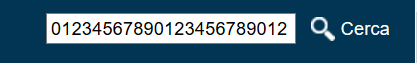
\includegraphics[scale=0.80]{C:/Users/elepo/Desktop/UNI/WIM/ANALISI_SITO/Relazione/sez/ricerca.png}
           \caption{Barra di ricerca}
           \end{center}
  \end{figure}
\end{center}
Per quanto riguarda invece la scelta dei colori, invece, la barra è bianca è lo sfondo dietro blu: il contrasto è abbastanza evidente e rende visibile la barra.\\
Un aspetto positivo consiste nel fatto che esiste la possibilità di effettuare una ricerca avanzata, la quale aggiunge filtri alla ricerca corrente (anno scolastico, opzioni di visualizzazione, numero di risultati per pagina).\\
\begin{center}
\begin{figure}[h!]
           \begin{center}
           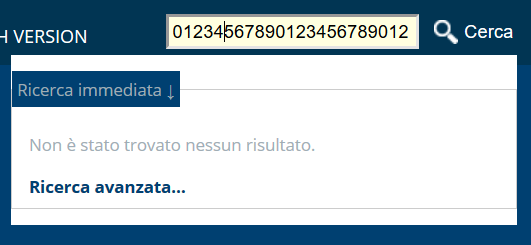
\includegraphics[scale=0.80]{C:/Users/elepo/Desktop/UNI/WIM/ANALISI_SITO/Relazione/sez/ricerca2.png}
           \caption{Ricerca avanzata}
           \end{center}
  \end{figure}
\end{center}
Una volta eseguita una ricerca (che sia basilare o avanzata non importa) i risultati sono visualizzati ad elenco, in un formato all'incirca similare a quello proposto dal motore di ricerca Google (e questo è un fattore positivo perchè l'utente ci è abituato). Un aspetto negativo, però, consiste nel fatto che se non esistono corrispondenza non viene data alcuna spiegazione o suggerimento all'utente per indirizzarlo verso una ricerca proficua.

\begin{center}
\begin{figure}[h!]
           \begin{center}
           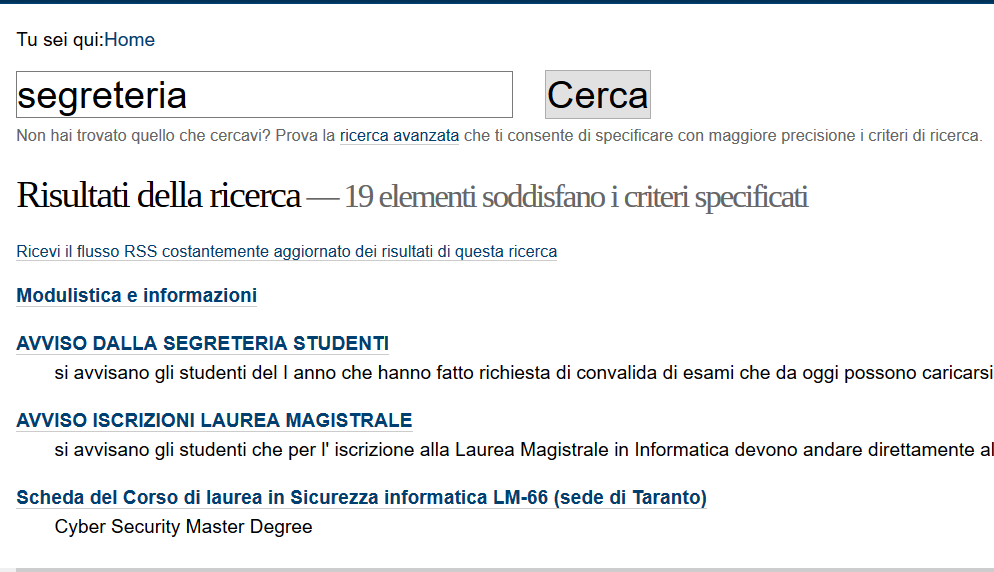
\includegraphics[scale=0.80]{C:/Users/elepo/Desktop/UNI/WIM/ANALISI_SITO/Relazione/sez/rr.png}
           \caption{Visualizzazione risultati ricerca}
           \end{center}
  \end{figure}
\end{center}